\documentclass{standalone}
\usepackage[dvipsnames]{xcolor}
\usepackage{tikz}
\usetikzlibrary{positioning, calc, shapes, fit, backgrounds}

\begin{document}
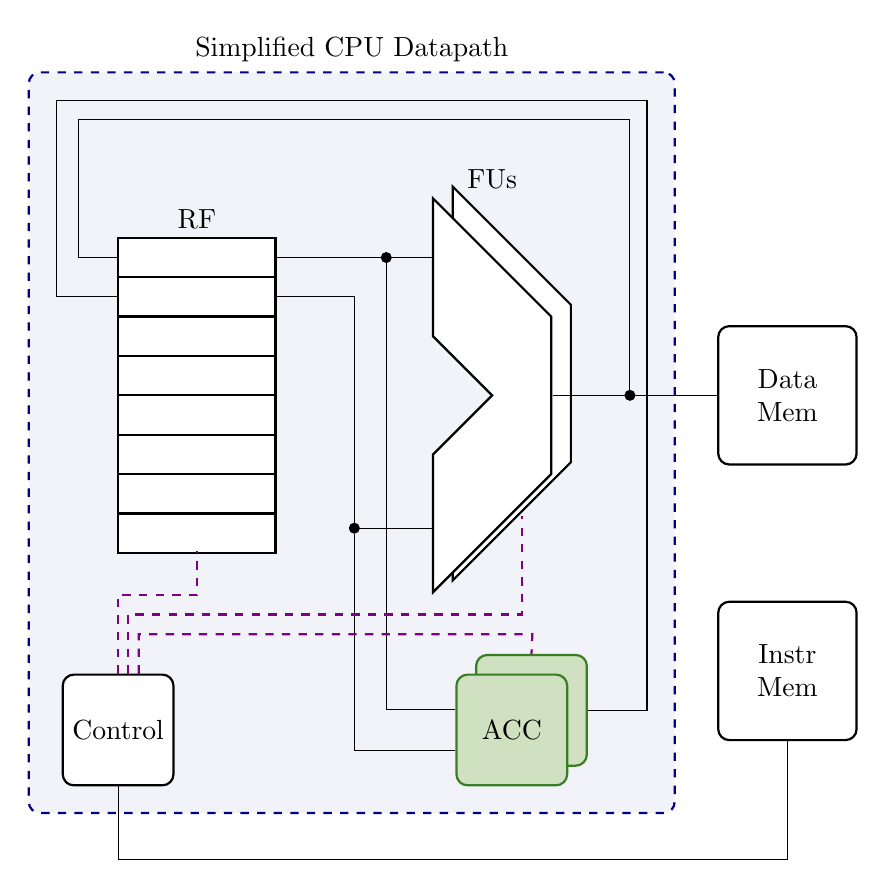
\begin{tikzpicture}
  \tikzstyle{coord}=[inner sep=0pt, outer sep=0pt, node distance=0pt]
  \tikzstyle{hwacc}=[rounded corners, draw=OliveGreen, fill=OliveGreen!20, thick, minimum size=40pt]
  \tikzstyle{control}=[draw=Purple, dashed, thick]
  \begin{scope}[name=datapath, local bounding box=dpathbb]

    % register file drawing
    \begin{scope}[name=rf, local bounding box=rfbb, shift={(0, -0.5)}]
      \node at (1,0) [anchor=south] {RF};
      \draw[fill=white, thick] (0,0) rectangle (2, -4);
      \foreach \i in {1,...,8} {
        \node (rfout\i) at (2, -0.5*\i+0.25) [coord] {};
        \node (rfin\i) at (0, -0.5*\i+0.25) [coord] {};
        \draw[thick] (0, -0.5*\i) -- (2, -0.5*\i);
      }
    \end{scope}

    % functional units
    \begin{scope}[name=fu, local bounding box=fubb, shift={(4, 0)}]
      \node at (0.75, 0) [anchor=south] {FUs};
      \begin{scope}[shift={(0.25, 0.15)}]
      \draw [fill=white, thick] (0, 0) -- (0, -1.75) -- (0.75, -2.5) -- (0, -3.25) -- (0, -5) -- (1.5, -3.5) -- (1.5, -1.5) -- cycle;
      \end{scope}
      \begin{scope}
        \draw [fill=white, thick] (0, 0) -- node [coord] (alua) {} (0, -1.75) -- (0.75, -2.5) -- (0, -3.25) -- node [coord] (alub) {}
        (0, -5) -- (1.5, -3.5) -- node [coord] (alux) {} (1.5, -1.5) -- cycle;
      \end{scope}
    \end{scope}

    % connections
    \draw (rfout1)  -| (alua);
    \draw (rfout2) -| ($(alub)!0.5!(rfout8)$) node (rfconn1) [coord, circle, fill=black, minimum size=4pt] {} -| (alub);
    \draw (alux) -- ++(1, 0) node (dataconn) [coord, circle, fill=black, minimum size=4pt] {} -- ++(0, 3.5) -- ++(-7, 0) |- (rfin1);

    % controller
    \node (ctl) at (0, -6.75) [draw, rectangle, rounded corners, minimum size=40pt, thick, fill=white] {Control};

    % tightly coupled acc
    \node (hwacc2) at (5.25, -6.5) [hwacc] {};
    \node (hwacc1) at (5, -6.75) [hwacc] {ACC};

    % accelerator connections
    \draw (hwacc2.east) -- ++(0.75, 0) -- ++(0, 7.75) -- ++(-7.5, 0) |- (rfin2);
    \draw (rfconn1) |- (hwacc1.200);
    \node (rfconn2) at (rfout1) [coord, circle, fill=black, minimum size=4pt, xshift=40] {};
    \draw (rfconn2) |- (hwacc1.160);
  \end{scope}

  \node (datamem) at (8.5, -2.5) [rounded corners, draw, thick, minimum size=50pt, align=center] {Data\\ Mem};
  \node (instmem) at (8.5, -6) [rounded corners, draw, thick, minimum size=50pt, align=center] {Instr\\ Mem};
  \draw (dataconn) -| (datamem.west);
  \draw (instmem.south) -- ++(0, -1.5) -| (ctl.south);

  % control lines
  \draw[control] (ctl.80) -- ++(0, 0.75) -- ++(5, 0) -- ++(0, 1.25);
  \draw[control] (ctl.90) -- ++(0, 1) -- ++(1, 0) -- ++(0, 0.55);
  \draw[control] (ctl.70) -- ++(0, 0.5) -- ++(1, 0);
  \draw[control] (ctl.70) -- ++(0, 0.5) -- ++(5, 0) -- (hwacc2.north);


  \begin{scope}[on background layer]
    \node [fit=(dpathbb), draw=NavyBlue, fill=NavyBlue!5, rounded corners, dashed, thick, inner sep=10pt,
    label={90:Simplified CPU Datapath}] {};
  \end{scope}
\end{tikzpicture}
\end{document}